%-----------------------------------------
% Note: Use pdflatex to process this file.
%-----------------------------------------

\documentclass{book}

\usepackage{graphicx}
\usepackage{moreverb}
\usepackage{amsmath}
\usepackage{alltt}
\usepackage{rotating}
\usepackage{subcaption}
\usepackage{toc}
\usepackage{xspace}
\usepackage{makeidx}
\usepackage{multirow}
\usepackage{booktabs}   % For table layouts
\usepackage{longtable}


\usepackage[T1]{fontenc}   % so _, <, and > print correctly in text.
\usepackage[strings]{underscore}    % to use "_" in text
\usepackage[pdftex,colorlinks=true]{hyperref}  % This must be the last package

\newcommand{\extref}[1]{$\S$\ref*{#1}}   % No hyperlink. For external refs. \extref
\newcommand{\comma}{\> ,}
\newcommand{\period}{\> .}
\newcommand{\wt}{\widetilde}
\newcommand{\grv}{\textasciigrave}
\newcommand{\hyperbf}[1]{\textbf{\hyperpage{#1}}}
\newcommand{\Ss}{\(^*\)}
\newcommand{\Dd}{\(^\dagger\)}

\newcommand{\AND}{&& \hskip -17pt\relax}
\newcommand{\CR}{\\}
\newcommand{\CRNO}{\nonumber \\}
\newcommand{\dstyle}{\displaystyle}

\newcommand{\Begineq}{\begin{equation}}
\newcommand{\Endeq}{\end{equation}}
\newcommand{\NoPrint}[1]{}

\newcommand{\pow}[1]{\cdot 10^{#1}}
\newcommand{\Bf}[1]{{\bf #1}}
\newcommand{\bfr}{\Bf r}

\newcommand{\bmad}{{\sl Bmad}\xspace}
\newcommand{\tao}{{\sl Tao}\xspace}
\newcommand{\mad}{{\sl MAD}\xspace}
\newcommand{\cesr}{{\sl CESR}\xspace}

\newcommand{\sref}[1]{\S\ref{#1}}
\newcommand{\Sref}[1]{Sec.~\sref{#1}}
\newcommand{\cref}[1]{Chapter~\ref{#1}}

\newcommand{\Newline}{\hfil \\ \relax}

\newcommand{\eq}[1]{{(\protect\ref{#1})}}
\newcommand{\Eq}[1]{{Eq.~(\protect\ref{#1})}}
\newcommand{\Eqs}[1]{{Eqs.~(\protect\ref{#1})}}

\newcommand{\vn}{\ttcmd}           % For variable names
\newcommand{\vni}{\ttcmdindx}
\newcommand{\cs}{\ttcmd}           % For code source
\newcommand{\cmd}{\ttcmd}          % For Unix commands
\newcommand{\rn}{\ttcmd}           % For Routine names
\newcommand{\tn}{\ttcmd}           % For Type (structure) names
\newcommand{\bn}[1]{{\bf #1}}       
\newcommand{\toffset}{\vskip 0.01in}
\newcommand{\rot}[1]{\begin{rotate}{-45}#1\end{rotate}}

\newcommand{\data}{{\mbox{data}}}
\newcommand{\reference}{{\mbox{ref}}}
\newcommand{\model}{{\mbox{model}}}
\newcommand{\base}{{\mbox{base}}}
\newcommand{\design}{{\mbox{design}}}
\newcommand{\meas}{{\mbox{meas}}}
\newcommand{\var}{{\mbox{var}}}

\newcommand\ttcmd{\begingroup\catcode`\_=11 \catcode`\%=11 \dottcmd}
\newcommand\dottcmd[1]{\texttt{#1}\endgroup}

\newcommand\ttcmdindx{\begingroup\catcode`\_=11 \catcode`\%=11 \dottcmdindx}
\newcommand\dottcmdindx[1]{\texttt{#1}\endgroup\index{#1}}

\newcommand{\St}{$^{st}$\xspace}
\newcommand{\Nd}{$^{nd}$\xspace}
\newcommand{\Th}{$^{th}$\xspace}
\newcommand{\B}{$\backslash$}
\newcommand{\W}{$^\wedge$}

\newcommand{\cbar}[1]{\overline C_{#1}}

\newlength{\dPar}
\setlength{\dPar}{1.5ex}

\newenvironment{example}
  {\vspace{-3.0ex} \begin{alltt}}
  {\end{alltt} \vspace{-2.5ex}}

\newcommand\Strut{\rule[-2ex]{0mm}{6ex}}

\newenvironment{Itemize}
  {\begin{list}{$\bullet$}
    {\addtolength{\topsep}{-1.5ex} 
     \addtolength{\itemsep}{-1ex}
    }
  }
  {\end{list} \vspace*{1ex}}

\newcommand{\Section}[1]{\section{#1}\indent\vspace{-3ex}}

\newcommand{\SECTION}[1]{\section*{#1}\indent\vspace{-3ex}}

% From pg 64 of The LaTex Companion.

\newenvironment{ventry}[1]
  {\begin{list}{}
    {\renewcommand{\makelabel}[1]{\textsf{##1}\hfil}
     \settowidth{\labelwidth}{\textsf{#1}}
     \addtolength{\itemsep}{-1.5ex}
     \addtolength{\topsep}{-1.0ex} 
     \setlength{\leftmargin}{5em}
    }
  }
  {\end{list}}


\setlength{\textwidth}{6.25in}
\setlength{\oddsidemargin}{0.25in}
\setlength{\evensidemargin}{0.00in}
\setlength{\textheight}{8.5in}
\setlength{\topmargin}{0in}

\renewcommand{\textfraction}{0.1}
\renewcommand{\topfraction}{1.0}
\renewcommand{\bottomfraction}{1.0}

\makeindex

\begin{document}

\index{lattice!model|see{model lattice}}
\index{lattice!design|see{design lattice}}
\index{lattice!base|see{base lattice}}

\thispagestyle{empty}

\begin{flushright}
\large
Revision: July 16, 2021 \\
\end{flushright}

\vfill

{
\begin{center}
\resizebox{1.8cm}{!}{\Huge \sf\bf The} \\
\vskip 0.2in

\includegraphics[width=10cm]{tao-logo.pdf} \\
\vskip 0.3in
\resizebox{4.4cm}{!}{\Huge \sf\bf Manual} \\
\vskip 0.4in
{\huge \sf\bf David Sagan} \\
\end{center}
}

\vfill
\break


%----------------------------------------------------------------
{
\setlength{\parskip}{\dPar}
\setlength{\parindent}{0ex}
}

%----------------------------------------------------------------

\cleardoublepage
\phantomsection 
\pdfbookmark[0]{Contents}{Contents}
\pdfbookmark[1]{Table of Contents}{toc} 
\tableofcontents


\cleardoublepage
\phantomsection 
\pdfbookmark[1]{List of Figures}{LoF} 
\listoffigures


\cleardoublepage
\phantomsection 
\pdfbookmark[1]{List of Tables}{LoT} 
\listoftables

%----------------------------------------------------------------
\setlength{\parskip}{\dPar}
\setlength{\parindent}{0ex}

%----------------------------------------------------------------

\chapter{Overview: Starting and Running Tao}
\label{c:overview.tao}

%----------------------------------------------------------------
\section{Tao Setup}
\label{s:obtaining}

Instructions for obtaining and for setting up \tao can be found at:
\begin{example}
  www.lepp.cornell.edu/bmad/
\end{example}

%----------------------------------------------------------------
\section{Tao Tutorial}
\label{s:tutorial}

This manual is organized more as a reference guide than as a tutorial so for an introduction
to \tao (and \bmad) there is a link on the web page at:
\begin{example}
  www.lepp.cornell.edu/bmad/tao.html
\end{example}

%-----------------------------------------------------------------
\section{Initialization from the Command Line}
\index{command line}
\label{s:command.line} 

The syntax of the command line for running \tao is:
\begin{example}
  EXE-DIRECTORY/tao \{OPTIONS\}
\end{example}
where \vn{EXE-DIRECTORY} is the directory where the tao executable lives. If this directory is
listed in your \vn{PATH} environmental variable then the directory specification may be omitted.
The optional arguments are:
%
\begin{description}
%
\item[\vn{-beam <beam_file>}] \Newline
Overrides the \vn{beam_file} (\sref{s:init.global}) specified in the
\tao initialization file.
%
  \item[\vn{-beam_all <all_beam_file>}] \Newline
Overrides the \vn{beam_all_file} (\sref{s:beam.init}) specified in the
\vn{tao_beam_init} namelist.
%
\item[\vn{-beam_init_file_name <file_name>}] \Newline
Overrides the \vn{beam_init%file_name} (\sref{s:beam.init}) specified in the
\vn{tao_beam_init} namelist.
%
\item[\vn{-building_wall <wall_file>}] \Newline
Overrides the \vn{building_wall_file} (\sref{s:init.global}) 
specified in the \tao initialization file.
%
\item[\vn{-data <data_file>}] \Newline
Overrides the \vn{data_file} (\sref{s:init.global}) specified in the
\tao initialization file.
%
\item[\vn{-disable_smooth_line_calc}] \Newline
Disable computation of the ``smooth curves'' used in plotting. 
This can be used to speed up \tao as discussed in \sref{s:plot.data}.
%
\item[\vn{-geometry <width>x<height>}] \Newline
Overrides the plot window geometry. \vn{<width>} and \vn{<height>}
are in Points. This is equivalent to setting \vn{plot_page%size}
in the \vn{tao_plot_page} namelist \sref{s:init.plot}.
%
\item[\vn{-hook_init_file}] \Newline
Specifies an input file for customized versions of Tao. Default file
name is \vn{tao_hook.init}.
%
\item[\vn{-init <tao_init_file>}] \Newline
replaces the default \tao initialization file name
(\vn{tao.init}). Note: A \tao initialization file is actually not
needed. If no \tao initialization file is used, the use of the
\vn{-lat} switch is mandatory and \tao will use a set of default plot
templates for plotting.
%
\item[\vn{-lat <bmad_or_xsif_lattice_file>}] \Newline
Overrides the \vn{design_lattice}
lattice file specified in the \tao initialization file
(\sref{s:init.lat}). Example:
\begin{example}
  tao -init my.init -lat slac.xsif
\end{example}
If there is more than one universe and the universes have different
lattices, separate the different lattice names using a "|" character.
Do not put any spaces in between. Example:
\begin{example}
  tao -lat xsif::slac.lat|cesr.bmad
\end{example}
%
\item[\vn{-log_startup}]
If there is a problem with \tao is started, \vn{-log_startup} can be used
to create a log file of the initialization process.
%
\item[\vn{-no_stopping}] \Newline
For debugging purposes. Prevents \tao from stopping where there is a fatal error.
%
\item[\vn{-noinit}] \Newline
Suppresses use of a \tao initialization file. In this case the use of
the \vn{-lat} switch is mandatory and \tao will use a set of default
plot templates for plotting.
%
\item[\vn{-noplot}] \Newline
Suppresses the opening of the plot window.
%
\item[\vn{-plot <plot_file>}] \Newline
Overrides the \vn{plot_file} (\sref{s:init.global}) specified in the
\tao initialization file.
%
\item[\vn{-prompt_color}] \Newline
Sets the prompt string color to Blue. For different colors, use the
\vn{set global prompt_color} command (\sref{s:set}).
%
\item[\vn{-rf_on}]
Leaves \vn{rfcavity} elements on. Normally \tao turns off these elements
since Twiss and dispersion calculations do not make sense with them on.
%
\item[\vn{-slice_lattice <element_list>}]
If present, discard from the lattice all lattice elements that are not in the \vn{<element_list>}.
Overrides the setting of \vn{design_lattice(i)%slice_lattice}.
%
\item[\vn{-startup <startup_command_file>}]
Overrides the \vn{startup_file} (\sref{s:init.global}) specified in the
\tao initialization file.
%
\item[\vn{-var <var_file>}] \Newline
Overrides the \vn{var_file} (\sref{s:init.global}) specified in the
\tao initialization file.

\end{description}

%----------------------------------------------------------------
\section{Initializing Tao}
\index{initializing!files}
\label{s:initializing}

Initialization occurs when \tao is started. Initialization information is stored in one or more
files as discussed in Chapter \sref{c:init}. If no initialization files are found. \tao uses a
default initialization.

%----------------------------------------------------------------
\section{Command Line Mode and Single Mode}
\label{s:modes}

After \tao is initialized, \tao interacts with the user though the command line. \tao has two modes
for this. In \vn{command line} mode, which is the default mode, \tao waits until the the \vn{return}
key is depressed to execute a command. Command line mode is described in Chapter~\sref{c:command}. 

In \vn{single} mode, single keystrokes are interpreted as commands. \tao can be set up so that in
\vn{single mode} the pressing of certain keys increase or decrease variables. While the same effect
can be achieved in the standard \vn{line mode}, \vn{single mode} allows for quick adjustments of
variables. See Chapter~\sref{c:single} for more details.

%-----------------------------------------------------------------
\section{Lattice Calculations}
\index{lattice calculaitons}
\label{s:lat.calc.overview} 

By default \tao recalculates lattice parameters and does tracking of particles after each command.
The exception is for commands that do not change any parameter that would affect such calculations
such as the \vn{show} command. See \sref{s:lat.calc} for more details. If the recalculation takes a
significant amount of time, the recalculation may be suppressed using the \vn{set global
lattice_calc_on} command (\sref{s:set.global}) or the \vn{set universe} command
(\sref{s:set.universe}).

%-----------------------------------------------------------------
\section{Command Files and Aliases}
\index{command files}
\label{s:command.files} 

Typing repetitive commands in command line mode can become tedious. \tao has two constructs to
mitigate this: Aliases and Command Files. 

Aliases are just like aliases in Unix. See Section~\sref{s:alias} for more details.

Command files are like Unix shell scripts. A series of commands are
put in a file and then that file can be called using the \vn{call}
command (\sref{s:call}).

\tao will call a command file at startup. The default name of this startup file is \vn{tao.startup}
but this name can be changed (\sref{s:format}).

Do loops (\sref{s:do}) are allowed with the following syntax:
\begin{example}
  do <var> = <begin>, <end> \{, <step>\} 
    ...
    tao command [[<var>]]
    ...
  enddo
\end{example}
The \vn{<var>} can be used as a variable in the loop body but must be
bracketed ``[[<var>]]''.  The step size can be any integer positive or
negative but not zero.  Nested loops are allowed and command files can
be called within do loops.

\begin{example}
  do i = 1, 100
    call set_quad_misalignment [[i]] ! command file to misalign quadrupoles
    zero_quad 1e-5*2^([[i]]-1) ! Some user supplied command to zero quad number [[i]]
  enddo
\end{example}

To reduce unnecessary calculations, the logicals \vn{global%lattice_calc_on}
and \vn{global%plot_on} can be toggled from within the command file. Example
\begin{example}
  set global lattice_calc_on = F  ! Turn off lattice calculations
  set global plot_on = F          ! Turn off plot calculations
  ... do some stuff ...
  set global plot_on = T          ! Turn back on 
  set global lattice_calc_on = T  ! Turn back on
\end{example}
Additionally, the \vn{global%command_file_print_on} switch controls
whether printing is suppressed when a command file is called.

A \vn{end_file} command (\sref{s:end.file}) can be used to signal the
end of the command file.

The \vn{pause} command (\sref{s:pause}) can be used to temporarily
pause the command file.

%----------------------------------------------------------------
\section{Customizing Tao}
\label{s:cust.tao}

Custom code can be linked with \tao to extend \tao's capabilities. For example, \tao can be extended to
be used as an online model in a control system. See Chapter~\sref{c:custom.tao} for more details.

\chapter{GUI Installation}
\label{s:gui.install}

%-----------------------------------------------------------------
\section{Obtaining the Source Code}

Source code and documentation for \bmad, \tao and the GUI for \tao can be obtained, if needed, at
the \bmad web site at:
  \hfill\break \hspace*{0.3in} \url{https://www.classe.cornell.edu/bmad}

%-----------------------------------------------------------------
\section{Building Tao}
\label{s:building}

As a prerequisite, if not already available, \tao must be built before using the GUI. Build
instructions are available on the \bmad web site. There are two ways for the GUI scripts (written in
Python) to interact with Tao. One way is to use the \vn{pexpect} module which is a communications
layer that interfaces to \tao's command line interface. The other way is to use \vn{ctypes} (an
interface between Python and C) to communicate directly with the \tao subroutine library (the \tao
program is built by linking to the \tao library). 

The advantage of using \vn{ctypes} is that it is faster. The drawback is that \vn{ctypes} requires a
version of the \tao library that is \vn{shared object}. If you are using a \bmad
``\vn{Distribution}'' (a package that is downloaded from the Web containing \bmad, \tao, associated
libraries, etc.), the default is {\em not} to build shared object libraries. This default can, of
course, be changed but if you do not have control of how things are built, you may have to use
\vn{pexpect}. To check if there is a shared object library built, issue the following command:
\begin{example}
  ls $ACC_ROOT_DIR/production/lib/libtao.*
\end{example}
[This assumes that you are not setting \vn{ACC_LOCAL_ROOT} as discussed in \Sref{s:e.vars}.]
In all cases you will see a file \vn{libtao.a}. This is a static library which is always built but
not of use. A file with an extension \vn{.so} (UNIX) or \vn{.dylib} (Mac) is a shared object library. 

%-----------------------------------------------------------------
\section{Python Requirements}

Minimum Python version for The GUI is Python 3.6.

The GUI depends upon a number of modules that may have to be downloaded:
\begin{example}
  tkinter
  ttk (may be called pyttk)
  pexpect         # If using pexpect instead of ctypes.
  matplotlib
  cycler
  ateutil
  tkagg
\end{example}
Note: The GUI uses the TkAgg backend for matplotlib. There may be a problem with Python finding the
TkAgg backend. On the mac, using macports, the solution is to install matplotlib with the
\vn{tkinter} variant. Something like:
\begin{example}
  sudo port uninstall py36-matplotlib           # May not be needed.
  sudo port install  py36-matplotlib +tkinter   # This is when using Python version 3.6
\end{example}
For more information see:
\begin{example}
  https://matplotlib.org/tutorials/introductory/usage.html#backends
\end{example}

If one of the modules is missing, python will generate an error message. For example:
\begin{example}
> python ../../gui/main.py
Exception in Tkinter callback
Traceback (most recent call last):
  File "/opt/local/Library/Frameworks/Python.framework/Versions/3.7/lib/
                            python3.7/tkinter/__init__.py", line 1705, in __call__
    return self.func(*args)
  File "../../gui/main.py", line 372, in param_load
    from tao_interface import tao_interface
  File "/Users/dcs16/Bmad/bmad_dist/tao/gui/tao_interface.py", line 4, in <module>
    from tao_pipe import tao_io
  File "/Users/dcs16/Bmad/bmad_dist/tao/python/tao_pexpect/tao_pipe.py", line 14, in <module>
    import pexpect
ModuleNotFoundError: No module named 'pexpect'
\end{example}
Notice that the last line shows that the pexpect module is needed.

How to install missing modules on the mac: [Note: The exact installation commands will depend upon
which version of python is being used. Use the "python --version" command to see what version you
are using.

Using macports and python 3.6:
\begin{example}
  sudo port install py36-tkinter
  sudo port install py36-pexpect
\end{example}

Using pip (or pip3):
\begin{example}
  sudo pip install pytkk
  sudo pip install pexpect
\end{example}

WARNING: it can be dangerous to use pip to install/modify modules in your system Python. A much
safer way to install the modules you need is to set up a python virtual environment.  On Linux, you
may also be able to find versions of the required modules in your system package manager, which are
tailored to your Linux distribution and will not break your system python.

%-----------------------------------------------------------------
\section{Environmental Variables}
\label{s:e.vars}
To run the GUI (or even to run \tao without the GUI), certain environmental varibles must be
set. This is the same initialization that is done when compiling \bmad and \tao. See your local Guru or the
\bmad web site for more details. To see if the environmental variables have been set, run the
\vn{accinfo} command.

It may be desireable to specify a local build tree as the place for the python scripts to find the
\tao executable or \tao shared object library. To accomplish this, set the environmental variable
\vn{ACC_LOCAL_ROOT} to the base directory of your local build tree.
\begin{example}
  export ACC_LOCAL_ROOT=/home/dcs16/bmad_dist
\end{example}

The standard place for the GUI script files is at:
\begin{example}
  "${ACC_ROOT_DIR}/tao/python/pytao/gui
\end{example}
When doing GUI development work, the default location can be changed by setting \vn{ACC_PYTHONPATH}. Example:
\begin{example}
  export ACC_PYTHONPATH="$ACC_LOCAL_ROOT/tao/python/pytao/gui"
\end{example}
[This assumes that \vn{ACC_LOCAL_ROOT} has been set.]  \vn{ACC_PYTHONPATH} must be set before \bmad
is initialized. That is, if \bmad is initialized in the \vn{.bashrc} file, \vn{ACC_PYTHONPATH} must
be initialized in the \vn{.bashrc} file before the \bmad initialization.

To check that \vn{PYTHONPATH} has the correct value use the command:
\begin{example}
  printenv |grep PYTHONPATH
\end{example}

%-----------------------------------------------------------------
\section{Installation Troubleshooting}
\label{s:gui.trouble}

Got error:
\begin{example}
  ImportError: cannot import name ‘_tkagg'
\end{example}

Solution: Uninstall and then reinstall matplotlib. For example, if using pip:
\begin{example}
  sudo pip uninstall matplotlib
  sudo pip install matplotlib
\end{example}

\chapter{GUI Startup}
\label{s:gui.startup}

%--------------------------------------------------------------
\section{Starting the GUI}

The GUI can be started from the system shell by executing the command
\begin{example}
  python -m pytao.gui
\end{example}
You can also specify any of the command line options that \tao supports.  For example,
\begin{example}
  python -m pytao.gui -init_file ~/bmad_dist/tao/examples/cesr/tao.init -rf_on
\end{example}
This will prefill the settings for \texttt{init_file} and \texttt{rf_on}. The GUI starts with the
window shown in Figure \ref{fig:startup}. From here, all of the command-line settings that Tao
supports can be set (settings that are left blank are omitted when Tao is started). The parameters
above the horizontal separator bar are \tao parameters and the parameters below the bar are GUI
specific parameters.

Towards the bottom of the window, below the horizontal separator, are some settings that are
specific to the GUI.  The "Interface to Tao" setting controls whether the ctypes or pexpect backend
for communicating with Tao will be used.  Below it, the "Shared Library" (if "Interface to Tao" is
set to "ctypes") or "Tao Executable" (if "Interface to Tao" is set to "pexpect") setting points the
GUI to the correct executable or shared object library to use.  In most cases, the GUI will prefill
this box by referencing the ACC_LOCAL_ROOT and ACC_ROOT_DIR environmental variables.

Finally, the font size can be set as desired. Hitting Enter/Return while the font size box is in
focus will adjust the font size of the startup window to give the user a sense of what the chosen
font size will look like.

Once all of the startup settings have been set, clicking "Start Tao" will initialize Tao and bring
the user to the main GUI window.

\begin{figure}
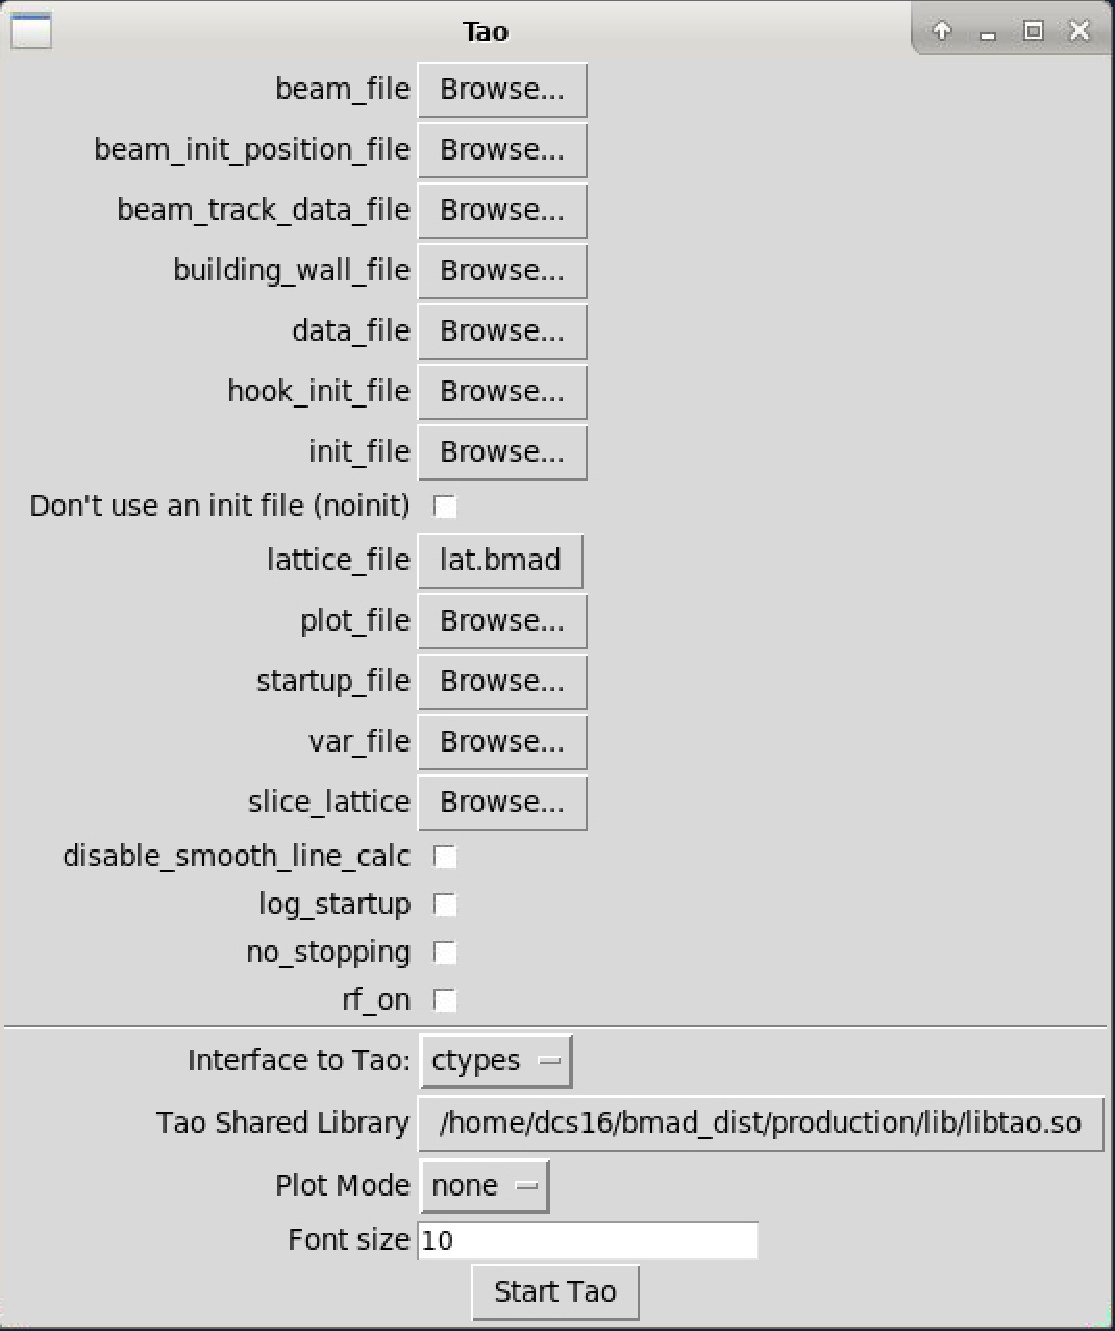
\includegraphics[width=8cm]{figures/startup.pdf}
\centering
\caption[The GUI startup window.]{The GUI startup window. In this example, the init file that tao should use has been specified.}
\label{fig:startup}
\end{figure}

%--------------------------------------------------------------
\section{GUI Initialization File}
\label{s:gui.init.file}

To speed up the initialization process, you can make an init file for the GUI.  This file should be called "gui.init", and it should be in the same directory from which you start the GUI.

gui.init should have each option on a separate line, and each option should be listed in the form "parameter:value".  For example, the text below would constitute a good gui.init file:
\begin{example}
  #MY GUI INIT FILE
  beam_file:/path/to/beam/file
  data_file:/path/to/data/file
  #THIS IS A COMMENT
  disable_smooth_line_calc:T
  rf_on:T
  tao_executable:/path/to/executable
\end{example}
For \tao specific parameters, The names in the \vn{gui.init} file correspond to the names in in the startup window
(\fig{fig:startup}). For GUI specific parameters (below the horizontal separator), replace blanks between words and
make all letters lower case. For example, ``\vn{Interface to Tao}'' in the startup window becomes \vn{interface_to_tao}
in the \vn{gui.init} file. Note: The startup window can be bypassed altogether by setting \vn{start_tao} in \vn{gui.init}
to \vn{True}.

The order in which you list options in gui.init is not important.

File paths should be specified in full to be safe, but you can specify paths relative to the directory from which you launch main.py.  For example, "/home/username/file", "subfolder/my_file", and "../../path/to/another/file" would all be acceptable file paths.  You can also use your environmental variables and "\textasciitilde{}", as in "\textasciitilde{}/Documents/my_file" and "\$DIST_BASE_DIR/tao/file".

For logical parameters, for example, "rf_on", Use T/F or True/False as the parameter's value.

You can also include comments with \#.  Anything after a \# character will be ignored.

To get a list of parameters that can be set in a \vn{gui.init} file, start Tao with the command
\begin{example}
  tao -help
\end{example}
The corresponding gui.init parameter is the Tao parameter with the leading dash "-" removed and a
colon ":" between the parameter and the parameter's value. 


\chapter{GUI Windows}

%-----------------------------------------------------------------
\section{Parameter Input}
\label{s:param.input}

In general, real parameter values can be set using expressions just like parameter values can be set
using expressions on the \tao command line.

%-----------------------------------------------------------------
\section{The Main GUI Window}
\label{s:gui.root.window}

\begin{figure}
\centering
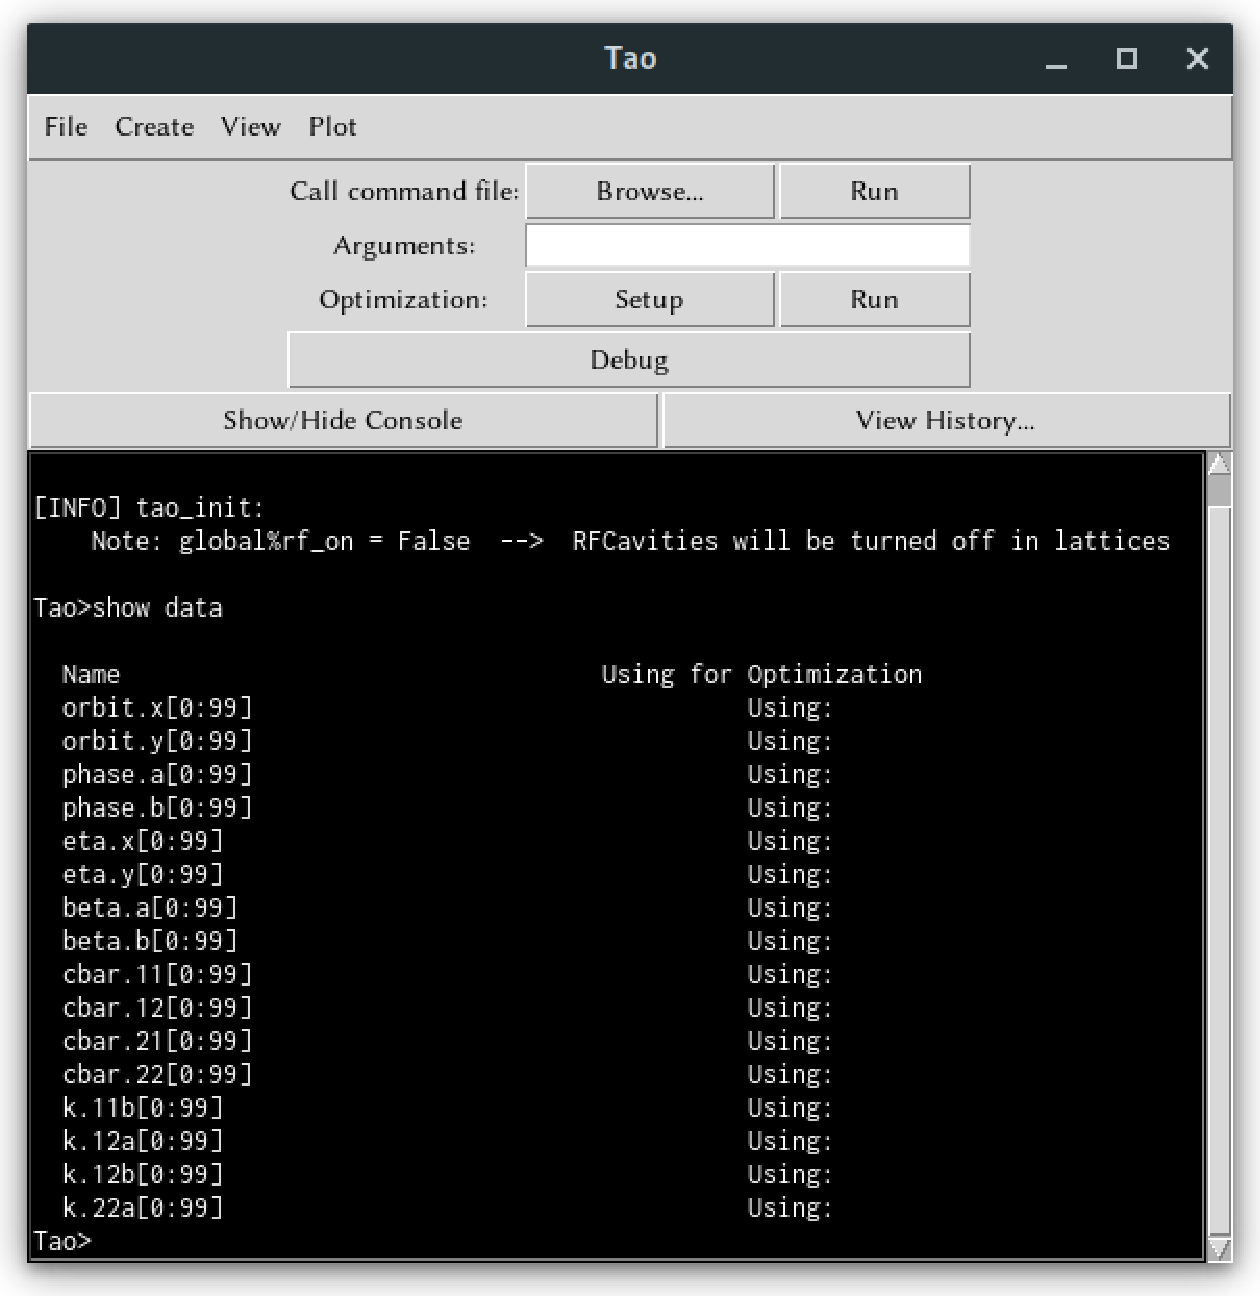
\includegraphics[width=8cm]{figures/root_window.pdf}
\caption[The main GUI window.]{The main GUI window, showing the results of \texttt{show data} on the console.}
\label{fig:root.window}
\end{figure}

The main window for the GUI is shown in Figure \ref{fig:root.window}.
From here, the user has access to all of the GUI's features.
Command files can be called by browsing for them and then clicking "Run", with arguments specified in the "Arguments" below.
In the future, the user will also be able to set up and run optimization routines from this window, although this feature is not currently available.

The main window also has a console, where commands can be run in Tao exactly like in regular Tao.
The console will also display warning messages if a command produces an error.

%-----------------------------------------------------------------
\section{Global Variables}
\label{s:gui.global.variables}

Global variables in Tao can be viewed and modified from the global variables window as shown in Figure \ref{fig:gui.global.variables}.
Once you have editted the global variables, clicking the "Set Global Variables" button will set the variables in Tao as appropriate.

\begin{figure}
\centering
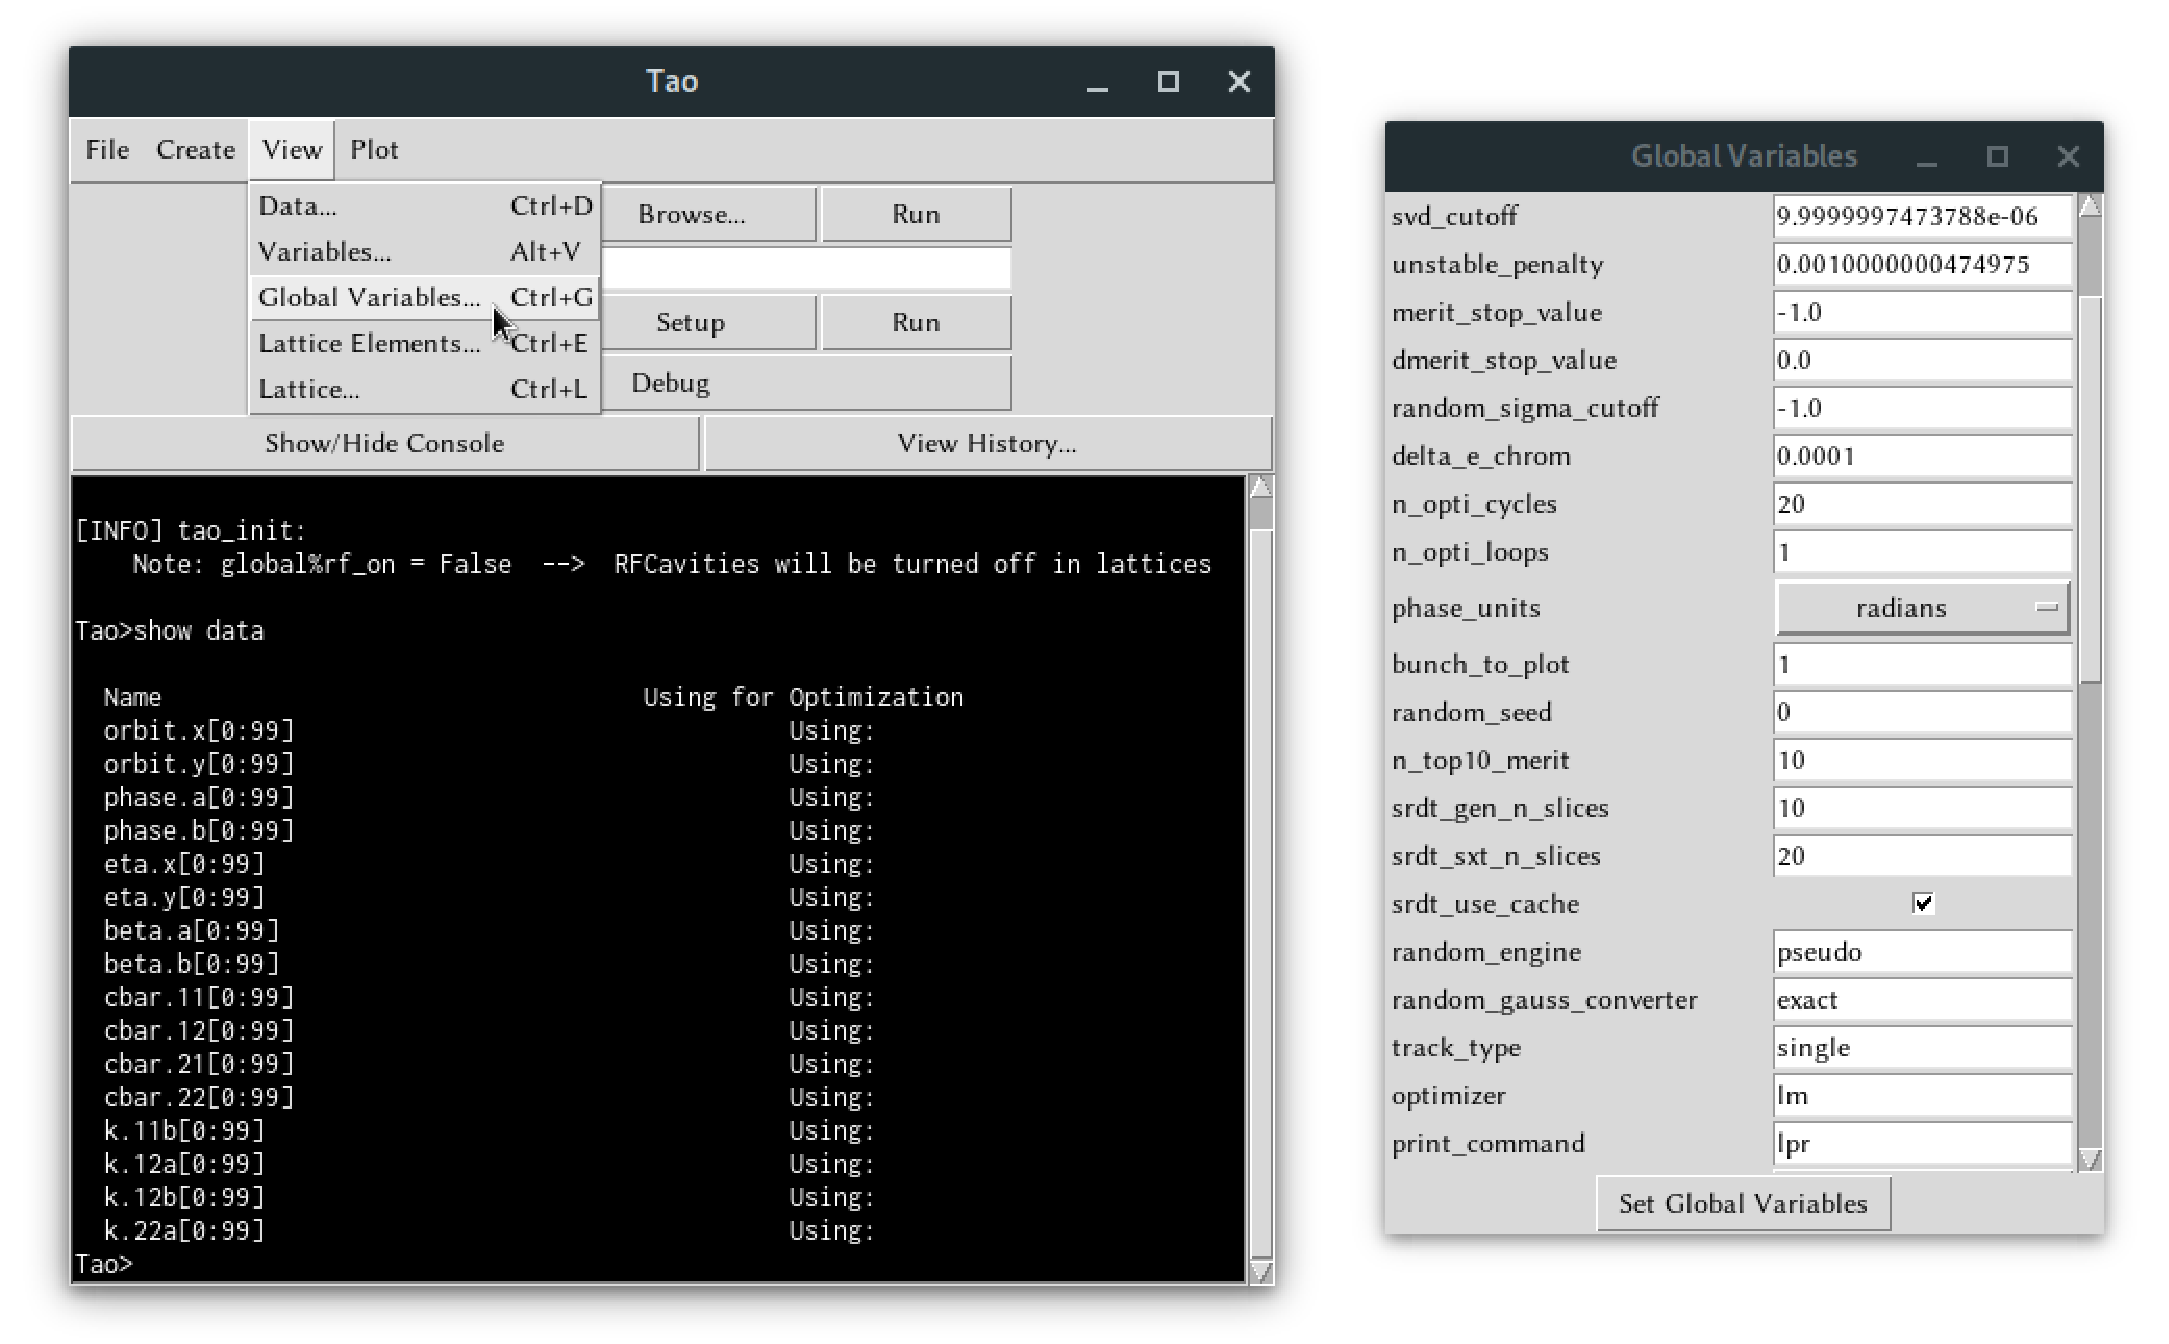
\includegraphics[width=10cm]{figures/globals.pdf}
\caption{View and edit global variables with the Global Parameters window.}
\label{fig:gui.global.variables}
\end{figure}


\chapter{Miscelaneous}

%-----------------------------------------------------------------
\section{Writing Namelists}
\label{s:gui.namelist}



\chapter{GUI Development}

%-----------------------------------------------------------------
\section{GUI Development} 
\label{s:develop}

%-----------------------------------------------------------------
\subsection{Profiling the GUI} 
\label{s:prfile}

To profile the GUI, first create a \vn{gui.init} file with:
\begin{example}
  skip_setup:T
  do_mainloop:F
\end{example}

then use the python script:
\begin{example}
  from pytao import gui
  import cProfile
  cProfile.run('gui.tao_root_window()', 'profile.dat')
\end{example}


%----------------------------------------------------------------
\begin{thebibliography}{XXXXXXX99}

\bibitem[Abell06]{b:rf.abell}
Dan Abell, ``Numerical computation of high-order transfer maps for rf cavities'',
Phys. Rev. ST Accel. Beams, vol. 9 (5) pp. 052001, (2006).

\bibitem[AML]{b:aml}
The Accelerator Markup Language / Universal Accelerator Project web page:
\hfill\break
\hspace*{0.3in}
\url{http://www.lepp.cornell.edu/~dcs/aml/}

\bibitem[Bater64]{b:batterman}
B.~Batterman, and H.~Cole,
``Dynamical Diffraction of X Rays by Perfect Crystals'',
Rev.\ Mod.\ Phys.,{\bf 36}, 3, pp.~ 681--717, (1964).

\bibitem[Berz89]{b:berz}
M. Berz, 
``Differential Algebraic Description of Beam Dynamics to Very High Orders,''
Particle Accelerators, Vol. 24, pp. 109-124, (1989).

\bibitem[Blas94]{b:blasdell}
R.~C.~Blasdell and A.~T.~Macrander, ``Modifications to the 1989 SHADOW
 ray-tracing code for general asymmetric perfect-crystal optics,''
Nuc.\ Instr.\ \& Meth. A {\bf 347}, 320 (1994).

\bibitem[Bmad]{b:bmad.web}
The Bmad web site:
\hfill\break
\hspace*{0.3in} \url{http://www.lepp.cornell.edu/~dcs/bmad}

\bibitem[Rio98]{b:del.rio}
Manuel Sanchez del Rio, ``Ray tracing simulations for crystal optics,''
Proc. SPIE 3448, Crystal and Multilayer Optics, {\bf 230} (1998). 

\bibitem[Brown77]{b:transport.appendix} 
K. L. Brown, F. Rothacker, D. C. Carey, and Ch. Iselin, ``TRANSPORT
Appendix,'' Fermilab, unpublished, (December 1977).

\bibitem[Chao93]{b:chao} 
Alexander Chao, {\em Physics of Collective Beam
Instabilities in High Energy Accelerators}, Wiley, New York (1993). 

\bibitem[Corbett99]{b:corbett}
J. Corbett and Y. Nosochkov, ``Effect of Insertion Devices in SPEAR--3,''
Proc. 1999 Part.\ Acc.\ Conf., p.~238, (1999).

\bibitem[Duff87]{b:leduff}
  J. Le Duff, \emph{Single and Multiple Touschek Effects}.
  Proc. CAS Berlin 1987,
  CERN 89-01,
  1987.

\bibitem[Forest02]{b:ptc}
E. Forest, F. Schmidt, E. McIntosh, 
{\it Introduction to the Polymorphic Tracking Code}, 
CERN–SL–2002–044 (AP), and KEK-Report 2002-3 (2002). 
Can be obtained at:
\hfill\break
\hspace*{0.3in}
\url{http://frs.web.cern.ch/frs/report/sl-2002-044.pdf}

\bibitem[Forest06]{b:geo.int}
`Etienne Forest, `Geometric integration for particle accelerators,''
J. Phys. A: Math. Gen. {\bf 39} (2006) 5321–5377.

\bibitem[Forest88]{b:quad.fringe}
E. Forest, J. Milutinovic, 
``Leading Order Hard Edge Fringe Fields Effects Exact in ($1+\delta$) and 
Consistent with Maxwell's Equations for Rectilinear Magnets,''
Nuc. Instrum. and Methods in Phys. Research A {\bf 269}, pp 474-482, (1988).

\bibitem[Forest98]{b:forest}
E. Forest, {\em Beam Dynamics: A New Attitude and Framework},
Harwood Academic Publishers, Amsterdam (1998).


\bibitem[Grote96]{b:maduser}
H. Grote, F. C. Iselin, {\it The MAD Program User's Reference Manual},
Version 8.19, CERN/SL/90-13 (AP) (REV. 5) (1996). 
Can be obtained at:
\hfill\break
\hspace*{0.3in}
\url{http://mad.home.cern.ch/mad} 

\bibitem[Healy86]{b:healy}
L. M. Healy, {\it Lie Algebraic Methods for Treating Lattice Parameter
Errors in Particle Accelerators}. Doctoral thesis, University of
Maryland, unpublished, (1986).

\bibitem[Helm73]{b:helm}
R. H. Helm, M. J. Lee, P. L. Morton, and M. Sands, ``Evaluation of Synchrotron
Radiation Integrals,'' IEEE Trans.~Nucl.~Sci. NS-20, 900 (1973).

\bibitem[Hoff06]{b:spin}
G.~Hoffstaetter, {\it Hight-Energy Polarized Proton Beams, A Modern View}, 
Springer. Springer Tracks in Modern Physics Vol~218, (2006).

\bibitem[Iselin94]{b:madphysics}
F. C. Iselin, {\it The MAD program Physical Methods Manual}, 
unpublished, (1994).  Can be obtained at: 
\hfill\break
\hspace*{0.3in}
\url{http://mad.home.cern.ch/mad}

\bibitem[Jowett87]{b:jowett} 
J. M. Jowett, ``Introductory Statistical Mechanics
for Electron Storage Rings,'' AIP Conf. Proc. 153, Physics of Part.\ Acc.,
M. Month and M. Dienes Eds., pp.~864, (1987).

\bibitem[Kohn95]{b:kohn}
V.~G.~Kohn, 
``On the Thcory of Reflectivitlby an X-Ray Multilaler Mirror''
physica status solidi (b), {\bf 187}, 61, (1995).

\bibitem[Press92]{b:nr}
W. Press, B. Flannery, S. Teukolsky, and W. Wetterling, {\em Numerical
Recipes in Fortran, the Art of Scientific Computing}, Second Edition,
Cambridge University Press, New York, (1992). \hfill \break
W. Press, B. Flannery, S. Teukolsky, and W. Wetterling, {\em Numerical
Recipes in Fortran90, the Art of Parallel Scientific Computing}, 
Cambridge University Press, New York, (1996).

\bibitem[Piwin98]{b:piwinski}
Anton Piwinski, \emph{The Touschek Effect in Strong Focusing Storage Rings}.
DESY 98-179, 1998.

\bibitem[Rosen94]{b:rosenzweig}
J. Rosenzweig and L. Serafini, ``Transverse Particle Motion in
Radio--Frequency Linear Accelerators,'' Phys Rev E, Vol. 49, p. 1599,
(1994).

\bibitem[Ruth87]{b:ruth} R. D. Ruth, ``Single-Particle Dynamics in
Circular Accelerators,'' in AIP Conference Proceedings {\bf 153}, {\em
Physics of Particle Accelerators}, pp.~152--235, M. Month and M. Dienes editors,
American Institute of Physics, New York (1987).

\bibitem[SAD]{b:sad} 
D.~Zhou and K.~Oide, ``Maps Used in SAD'' (unpublished).
Also see:
\hfill\break
\hspace*{0.3in} \url{http://acc-physics.kek.jp/SAD/}

\bibitem[Sagan03]{b:wiggler}
D. Sagan, J. Crittenden, and D. Rubin.
``A Symplectic Model for Wigglers,'' Part.\ Acc.\ Conf. (2003).

\bibitem[Sagan99]{b:coupling}
D. Sagan and D. Rubin ``Linear Analysis of Coupled Lattices,''
Phys.\ Rev.\ ST Accel.\ Beams {\bf 2}, 074001 (1999).
\hfill\break
\hspace*{20pt} 
\url{http://link.aps.org/doi/10.1103/PhysRevSTAB.2.074001}

\bibitem[Sagan06]{b:csr}
D. Sagan, ``An Efficient Formalism for Simulating the Longitudinal Kick from Coherent 
Synchrotron Radiation,'' Proc. Europ.\ Part.\ Accel.\ Conf. p. 2829 --- 31 (2006).

\bibitem[Storn96]{b:de}
R.~Storn, and K.~V.~Price, ``Minimizing the real function of the
ICEC'96 contest by differential evolution'' IEEE conf. on Evolutionary
Computation, 842-844 (1996).

\bibitem[Stoltz02]{b:boris}
P. H. Stoltz and J. R. Cary, ``Efficiency of a Boris--like Integration
Scheme with Spatial Stepping,'' Phys.\ Rev.\ Special Topics ---
Accel. \& Beams {\bf 5}, 094001 (2002).

\bibitem[Talman87]{b:talman} R. Talman, ``Multiparticle Phenomena and
Landau Damping,'' in AIP Conf.\ Proc.  {\bf 153}, {\em Physics of
Particle Accelerators}, pp.~789--834, M. Month and M. Dienes editors,
American Institute of Physics, New York (1987).

\bibitem[Tao]{b:tao}
D. Sagan, J. Smith, {\it The Tao Manual}.
Can be obtained at: \hfill\break
\hspace*{0.3in}
\url{http://www.lepp.cornell.edu/~dcs/bmad/tao_entry_point.html}

\bibitem[Rauben91]{b:tol}
T. Raubenheimer,
``Tolerances to Limit the Vertical Emittance in Future Storage Rings'', 
Particle Accelerators, 1991, {\bf 36}, pp.75-119. 
SLAC-PUB-4937 Rev., (1991).

\bibitem[Wiede99]{b:wiedemann}
H. Wiedemann, {\em Particle Accelerator Physics}, Springer, New York, 3rd Edition (2007). 

\bibitem[Wolski06]{b:wolski.coupling}
A.~Wolski,  ``Alternative approach to general coupled linear optics,''
Phys. Rev. ST Accel. Beams 9, 024001 (2006).

\bibitem[Wyckoff65]{b:wyckoff}
R. W. G. Wyckoff, {\em Crystal Structures}, Interscience Publ. (1965).

\bibitem[Schoon11]{b:xraylib} 
T. Schoonjans et al. ``The xraylib library for X-ray-matter
interactions. Recent developments,'' Spectrochimica Acta Part B: Atomic
Spectroscopy {\bf 66}, pp. 776-784 (2011).

\index{XSIF!reference}
\bibitem[Tenen01]{b:xsif}
P. Tenenbaum, ``LIBXSIF, A Stand alone Library for Parsing the Standard 
Input Format,'' Proc.\ 2001 Part.\ Acc.\ Conf.\ p. 3093 --- 95 (2001).
Documentation at
\hfill\break
\hspace*{0.3in} \url{http://www-project.slac.stanford.edu/lc/ilc/TechNotes/LCCNotes/PDF/LCC-0060%20rev.1.pdf}

\end{thebibliography}


\printindex

\end{document}
